\chapter{Kinematics of manipulators}
\begin{quotation}
    \noindent\textsf{
        In this chapter we will talk about \textit{kinematics of manipulators}. How we will see, they are totally different with respect to mobile robots: if for mobile robots we have a moving chassis mounted on wheels, on the other hand we have chains of links and joints. This is due to substancial mechanical difference among the two cateogories. We will give an introduction on the structure of such robots (joint, links, wrists...) and then we will describe the \textit{direct kinematics problem} and the \textit{inverse kinematics problem}.
    }
\end{quotation}
\minitoc

\section{Kinematic chains}
The \textbf{Kinematics} allows us to study the \textit{position, velocity and acceleration} of particular points of a multibody system independently from forces and torques that generated them. In order to describe the \textit{kinematic for manipulator} the definition of \textbf{kinematic chain} is needed.
\begin{definition}[Kinematic chain]
    A \textbf{kinematic chain (KC)} is a series of ideal arms/links connected by ideal joints.
\end{definition}
For our purposes a KC is only a geometric entity, we will not consider mass, inertia, friction and so on. More specifically:
\begin{itemize}
    \itemsep-0.3em
    \item \textit{links/arms} are idealized with geometric bars connecting two or more joints; 
    \item \textit{Joints} are idealized physical components allowing a relative motion among consecutive arms. Each joint provides a \textbf{degree of motion}.
\end{itemize}

\begin{figure}
    \centering
    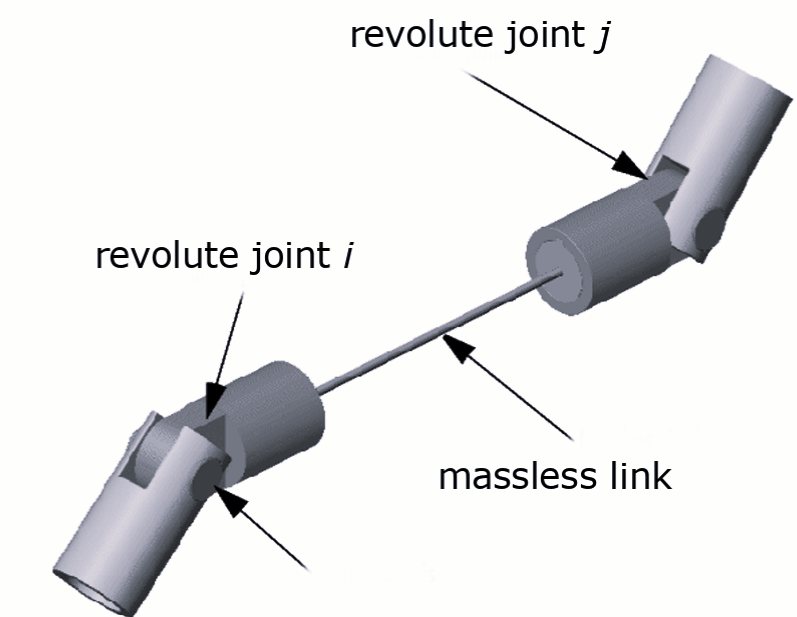
\includegraphics[scale=0.5]{img/joints_links.png}
    \caption{The robot joints are moved by actuators (eg. motors) and are connected by links/arm which are assumed to be massless}.
\end{figure}
\newpage
\subsection{Types of joints}
In the following we will consider two types of joints: 
\begin{enumerate}
    \itemsep-0.3em
    \item \textsf{Revolute (or Rotational) joints} which allows a \textbf{rotation} between the connected links; 
    \item \textsf{Prismatic (or Traslational) joints} which allows a \textbf{translation} between the connected links.
\end{enumerate}

\begin{figure}
    \centering
    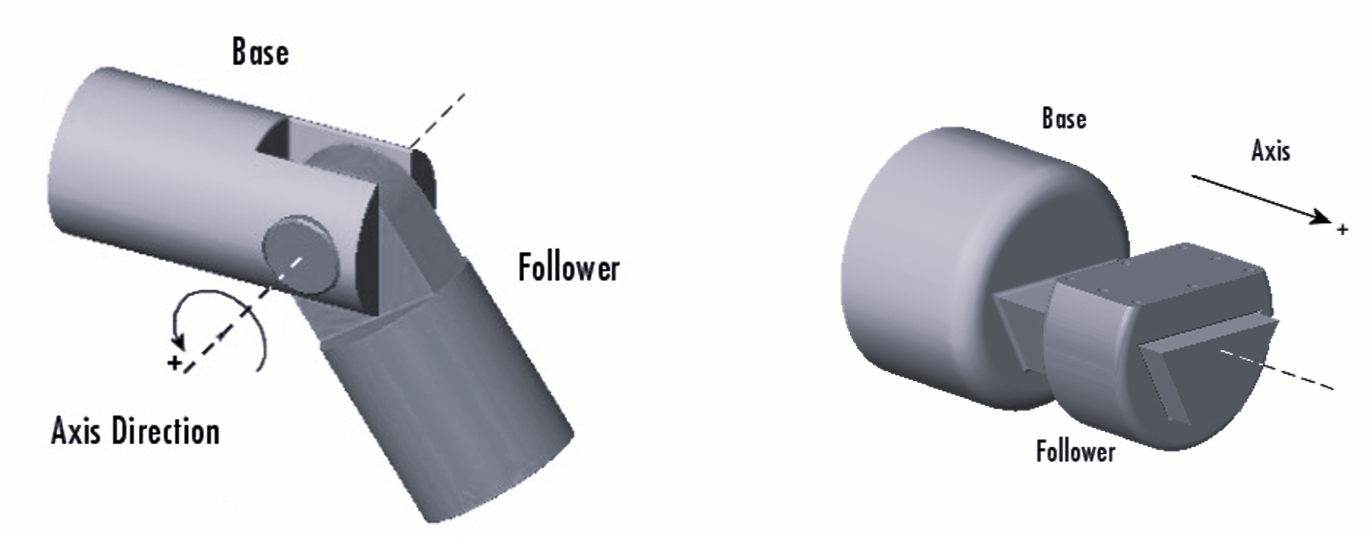
\includegraphics[scale=0.5]{img/joints_tyeps.png}
    \caption{Revolute and Prismatic joints. With a dashed line the direction of motion (axis) is indicated}
\end{figure}
According to the number of links we can find between any two joints, kinematic chains can be \textbf{open chains} or \textbf{closed chains}. In the former case there is only one link between any two links in a way joints and arms form a \textit{tree-like} structure; in the latter case there might be more than one link between any two joints, and in this case joints and arms are arranged in a \textit{cycle-like} structure.

\subsection{Graphical representation}
There are different types of graphical representations for kinematic chains, in the following we will use cylinders and boxes for joints, segment for links/arms. 

\begin{figure}
    \centering
    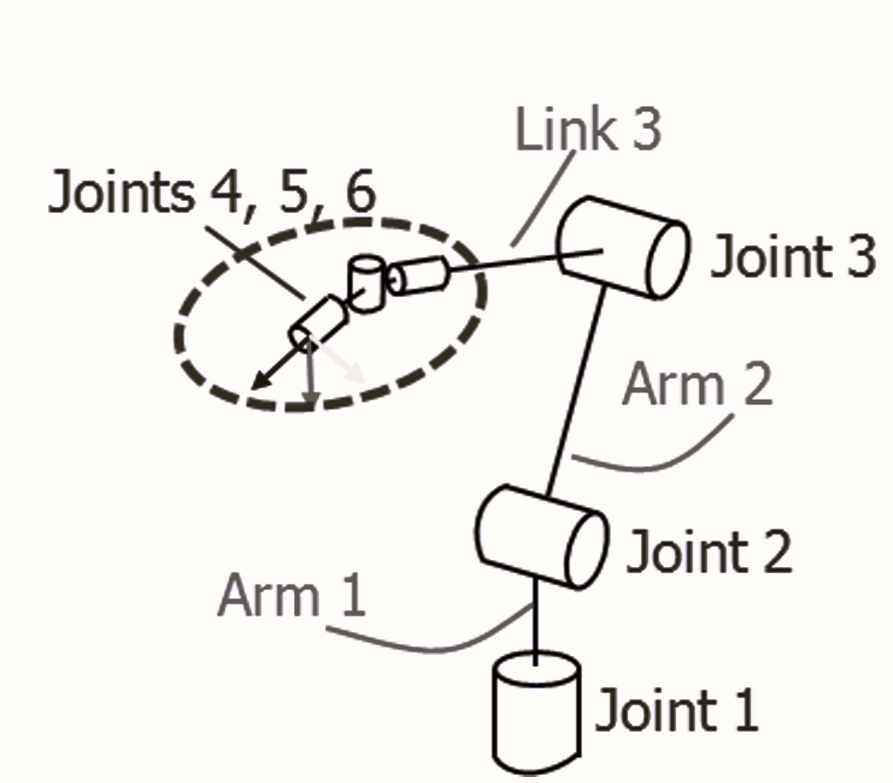
\includegraphics[scale=0.5]{img/KC_sample.png}
    \caption{Kinematic chain sample}
    \label{fig:KC_sample}
\end{figure}
More specifically \textit{\textbf{rotation joints}} are drawn in 3D has small cylinders withb the axes aligned along each rotation axis, in 2D they are drawn as small circles or small hourglasses.

\begin{figure}[h]
    \centering
    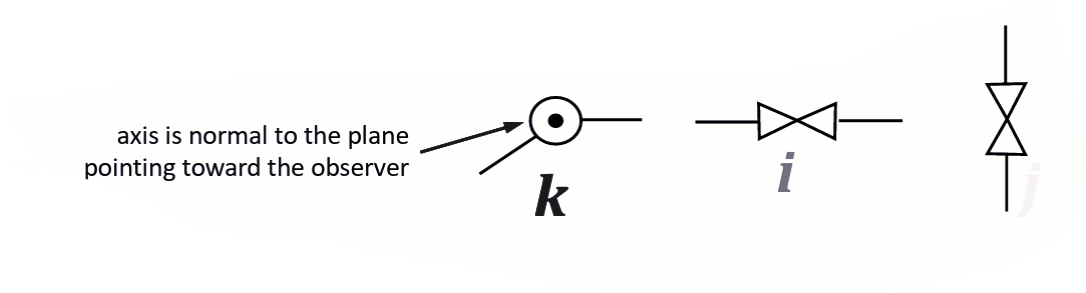
\includegraphics[scale=0.6]{img/rot_joints.png}
    \caption{2D-representation for revolute joints}
\end{figure}

At the opposite, \textit{\textbf{prismatic joints}} are represented as small boex with each axis aligned along the translation axis. On the other hand in 2D they are drawn as small squares with a point in their center, or as small rectangles showing the direction for the outcoming links.

\begin{figure}
    \centering
    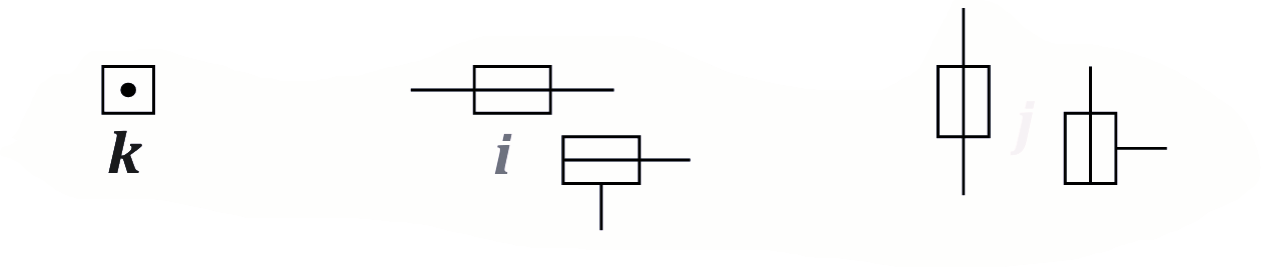
\includegraphics[scale=0.5]{img/transl_joints.png}
    \caption{2D representation of translational joints}
\end{figure}

\begin{figure}
    \centering
    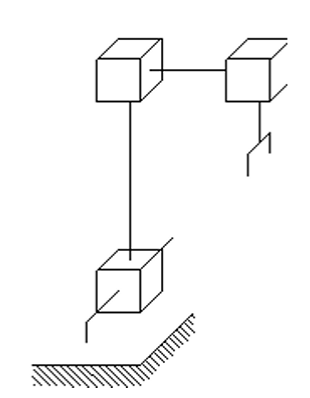
\includegraphics[scale=0.6]{img/transl_joints_3D.png}
    \caption{3D graphical representation for prismatic joints}
\end{figure}

\subsection{End-effector}
The \textbf{end-effector} (also called \textit{hand, gripper} or \textit{hand tool}) is the structure which is attached to the last link, and it is the one by which the task, for which that robot was introduced, can be executed. For the end effector a particular type of point is interesting, this is the \textbf{Tool Center Point (TCP)} and it is the baricenter of the hand, or better that ideal point that the robot software moves through the space. How we will see it is useful to attach to such a point a reference frame. \\
The graphical representation is used for the end-effector is a sort of fork. The end-effector can be of any type and we can draw and study the kineamtic chain without assuming the use of any particular hand.

\begin{figure}
    \centering
    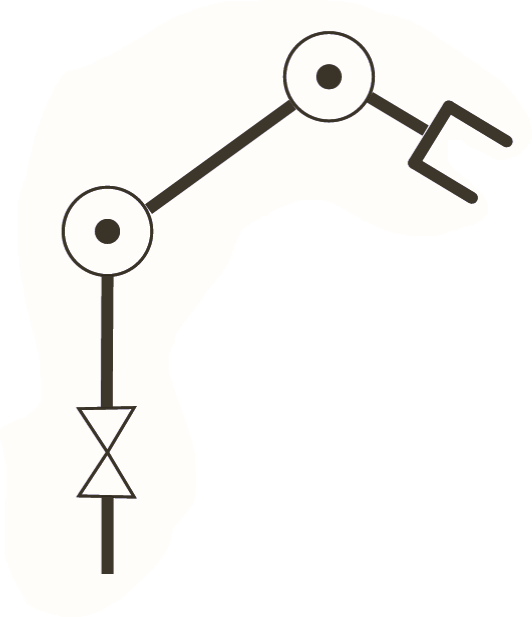
\includegraphics[scale=0.4]{img/endeff_graphical.png}
    \caption{End-effector graphical representation. Typically the TCP is assumed to be the center of the 'fork'}
\end{figure}




\section{Robot types}
An \textbf{Industrial manipulator} is usually composed by a \textbf{shoulder} and a \textbf{wrist}. The manipulators can be categorized according to the structure of their arms, which are based on the type of joints. We will indicate:
\begin{center}
    \underline{\textbf{R=revolute joint}}\\
    \underline{\textbf{P=Prismatic joint}}
\end{center}
A great number of robots can be obtain according the shoulder configuration, however in the industrial fields, few configurations are used which are more suitable for certain tasks instead of others. In the following \Cref{tab:manip_types} we are going to explore the most common structures giving their main characteristics.

\begin{longtable}{c c m{8cm}}
    \caption{Common types of manipulators}\\
    \hline
    \textbf{Robot type} & \textbf{Image} & \textbf{Description} \\
    \hline
    \endfirsthead

    \hline
    \textbf{Robot type} & \textbf{Image} & \textbf{Description} \\
    \hline
    \endhead

    \hline
    \endfoot

    \hline
    \endlastfoot\\
    \caption{Common types of manipulators}\label{tab:manip_types}\\

    \textbf{Cartesian Manipulator} & 
    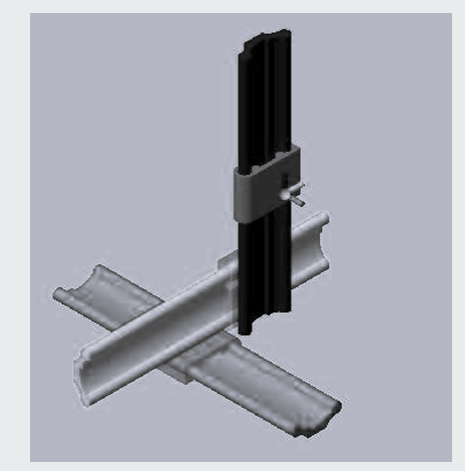
\includegraphics[width=3cm]{img/man_cart.png} & 
    In a \textbf{cartesian manipulator} the structure \texttt{(PPP)} is related to the shoulder structure. In this case the shoulder is composed of three prismatic joints, whose axis are mutually orthogonal. In this case, each degree of motion corresponds to a cartesian variable. We anticipate that the task space is a sort of \textit{parallelepiped}. Such robots have good accuracy, while regarding dexterity, it cannot be said the same. \\
    \hline
    \textbf{Cylindrical Manipulator} & 
    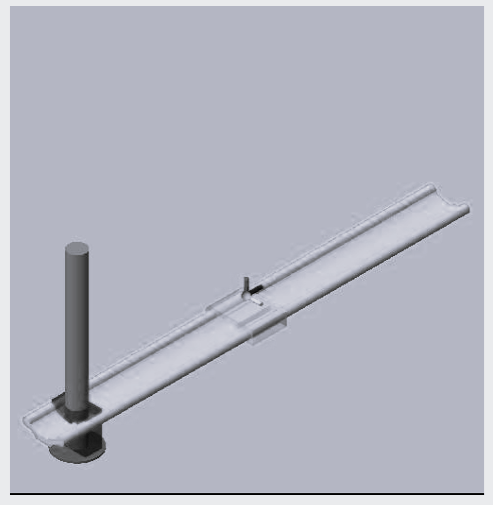
\includegraphics[width=3cm]{img/cyl_man.png} & 
    One rotoidal joint and two prismatic joints are the basic building blocks for the shoulder of a cylindrical manipulator. Each DOM (degree of motion) corresponds to a cylindrical coordinate. The \textit{task space} is a \textbf{cylindrical sector}. The horizontal prismatic joint allows reaching horizontal spaces; however, the accuracy decreases toward the arm ends. \\
\hline
    \textbf{Spherical Manipulator} & 
    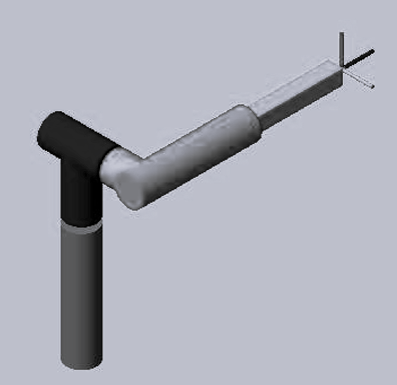
\includegraphics[width=3cm]{img/spherical_man.png} & 
    For a \textbf{polar (or spherical) manipulator}, the shoulder has two revolute joints followed by a prismatic one. Each DOM corresponds to a polar coordinate; here, the task is a spherical sector that may include parts of the floor to allow the manipulation of objects there located. The structure is less rigid compared to previous ones, and the accuracy reduces with the elongation of the prismatic arm. \\
\hline
    \textbf{SCARA \texttt{(RRP)}} & 
    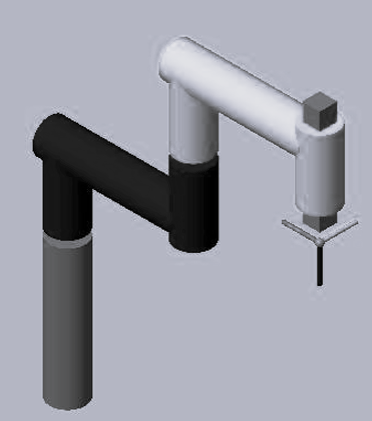
\includegraphics[width=3cm]{img/scara.png} & 
    It is a robot used for \textit{pick and place} applications. The shoulder has two revolute joints followed by one prismatic joint, all with \textbf{parallel vertical axes}. The tasks addressed by this robot are the manipulation of small components or little assembly tasks. \\
\hline
    \textbf{Antropomorphic} & 
    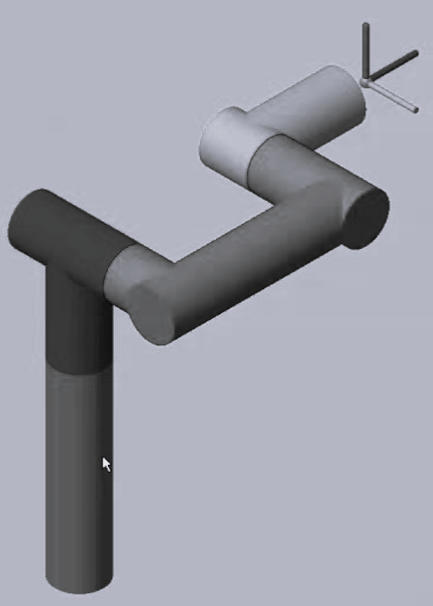
\includegraphics[width=3cm]{img/antrop_man.png} & 
    The shoulder is composed of \textbf{three revolute joints}: the first one is vertical, the others are \textbf{horizontal and parallel}. It is one of the most common structures in the industry since it is the robot having \textbf{the best dexterity}. \\
\hline
    \textbf{Parallel robots}&{
        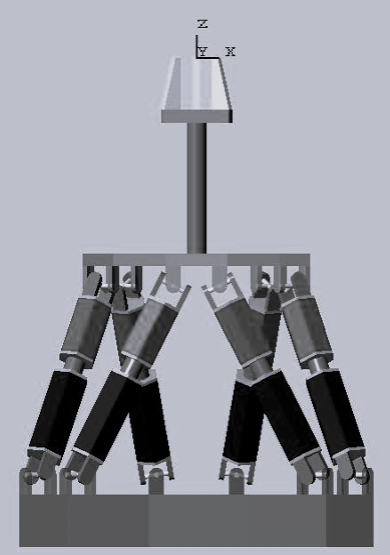
\includegraphics[width=3cm]{img/parallel_man.png}
    }&{
        Such a type of manipulators have joints and links forming a cycle-like structure. They are not covered in these notes. An example is showed in the figure aside.
    }\\
    
\end{longtable}
%------------------------------------------------------------


\section{Wrists}
The main scope of the \textbf{wrist} is to \textit{give an orientation} to the TCP. In fact, it can be said that the shoulder sets the \textbf{origin position}, while the \textbf{wrist} orients the TCP. \textit{Spherical wrists} are the most common. A wrist is said to be \textbf{spherical} if the three axes always intersect in a single point.Even if not spherical, due to its orientation function, the wrist is made up of \textbf{three rotational joints}.

\begin{figure}[h]
    \centering
    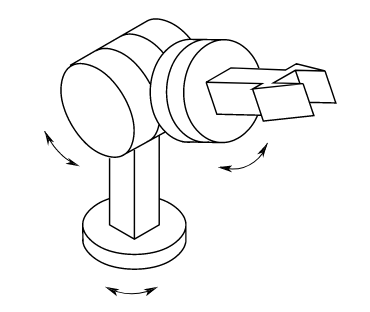
\includegraphics[scale=0.7]{img/polso.png}
    \caption{Spherical wrist}
\end{figure}
Taking into account a spherical joint, simplifies a lot the tractation of related topics of both manipulator kinematics and dynamics. Looking at the \Cref{fig:KC_sample} the wrist is the terminal part made up of joints 4,5,6.
 
\section{Direct Kinematics}
Many times in robotics there is the need to connect the "external world" to "robot world". In studying the kinematics of a manipulator the questions can arise are:
\begin{enumerate}
    \item Where is the end-effector given the information about the joints? (This is known as the \textbf{Direct kinematics problem}).
    \item What is the position of the joints to have in order to obtain a certain position of the end-effector? (This is known as the \textbf{Inverse kinematics problem})
\end{enumerate}
More specifically, the information about the joints are given by using \textbf{joint variables}, how we will see in explaining the Denavit-Hartemberg convention.

\begin{comment}
\begin{figure}[h]
    \centering
    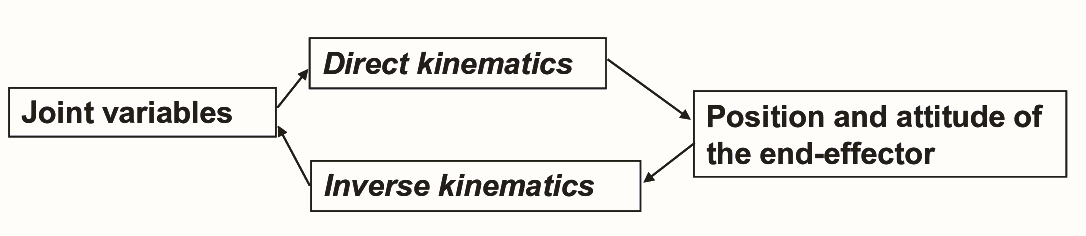
\includegraphics[scale=0.6]{img/direct_inverse_kinematics.png}
\end{figure}
\end{comment}

\begin{figure} [h]
    \centering
    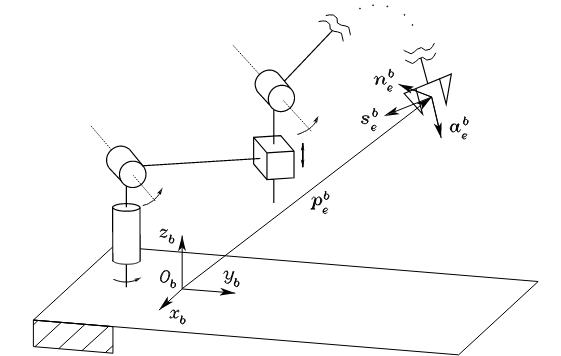
\includegraphics[scale=0.8]{img/kinematic_chain.png}
    \caption{Kinematic chain: joints and arms}
    \label{fig:chain}
\end{figure}
From now on, we are considering a manipulator consisting of $n+1$ links conected in an open chain through the use of $n$ joints\footnote{It is sufficient to think that for a joint is for two links.}.\\
With respect to the reference frame attached to the base of the robot $\mathcal{R}_b=\{O,x_b,y_b,z_b\}$ the \textbf{direct kinematic function} is expressed in term of the homogeneuous transformation matrix 
\begin{equation}
    \bb{T}_e^b(\bb{q})=\begin{bmatrix}
        \bb{n}_e^b(\bb{q})& \bb{s}_e^b(\bb{q})& \bb{a}_e^b(\bb{q})& \bb{p}_e^b(\bb{q})\\
        0&0&0&1
    \end{bmatrix}
    \label{eq:homtransform}
\end{equation}
where $\bb{q}$ is the vector containing the \textbf{joint variables} for the $n$ joints. While $\mathcal{R}_e=\{O_e,n_e,s_e,a_e\}$ is a reference frame related to the end-effect (this is chosen according to the specific task geometry). 
Some further clarification about $\mathcal{R}_e$. If the end-effector is a gripper the origin of the frame is put in the TCP, the unit vectors are: 
\begin{enumerate}
    \itemsep-0.3em
    \item $\bb{a}$ stands for \textbf{approach}, lays along the approach direction; 
    \item $\bb{s}$ stands for \textbf{sliding} lays along the sliding plane of the gripper jaws.
    \item $\bb{n}$ completes the right-handed frame.
\end{enumerate}
A first approach to use to obtain the \Cref{eq:homtransform} is by inspection  and using geometrical considerations. A more efficient and relatively \textit{effortless approach} is to use a systematic procedure. Things are made even more complicate when there are two or more closed kinematic chains. In the following we are going to briefly introduce the procedure for the case of \textit{open kinematic chain}. 

\subsection{Open-chain manipulators and Denavit-Hartemberg convention}
We have seen in \Cref{fig:chain} that we have $n+1$ links with $n$ number of joints. The Link 0 by convention is fixed to the ground, and (very important) \textbf{the actuation of the Link $i$ moves link $i$}. Moreover, for each link we attach a reference frame so that when link $i$ is actuated both the reference system and the link move.\\
Our objective is to relate the Link 0 with the Link $n$, looking for an homogeneous transformation between the frame $n$ and the frame $0$. This can be done in a recursive manner, computing for each link the relationship between the frame $i$ and the frame $i-1$ by mean of matrices $A_{i}^{i-1}$ where $i-1$ plays the role of fixed reference frame. At this point the \textit{solution of the direct kinematic problem} is obtained by post-multiplying the homogeneous transformation matrices. That is
\begin{equation}
    \bb{T}_n^0(\bb{q}) = 
        A_1^0(q_1)A_2^1(q_2)\dots{A_n^{n-1}(q_n)}
\end{equation}

Not rarely, the base and the end-effector frames does not coincide with the frames 0 and $n$, then the final $\bb{T}_e^b(\bb{q})$ is obtained as follows
\begin{equation}
    \bb{T}_e^b(\bb{q})=\bb{T}_0^bT_n^0(\bb{q})T_e^n 
\end{equation}

The matrices relating the base with the Link 0 and the frame $n$ with the end-effector frame are generally constant.\\
The \textbf{Denavit-Hartemberg convention} (DH convention) gives a systematic procedure to place the $n+1$ reference frames for each link and for obtaining the matrices $A^{i-1}_i$ for each link.

\begin{figure}
    \centering
    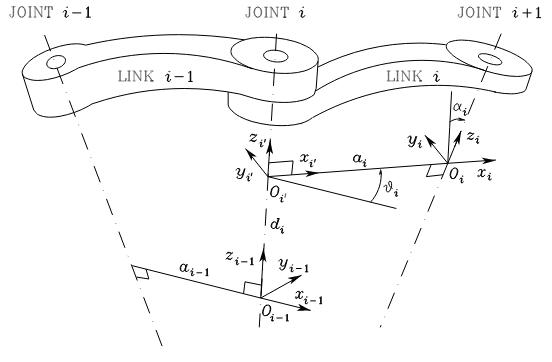
\includegraphics[scale=1]{img/DH_convention.png}
    \caption{\textbf{DH parameters}. The $z_{i}$ axis along the direction of motion for the related joint. $O_{i}$ is the intersection of ${z_i}$ with the common normal between $z_{i-1}$ and $z_{i}$, while $O_{i'}$ is the intersection between the common normal and $z_{i-1}$. $x_{i}$, ${x}_{i'}$ are chosen along the common normal from $i-1$ to $i$. The unit vectors $y_{i}$, ${y}_{i'}$ are to complete the right-handed reference frames.}
    \label{fig:DHparam}
\end{figure}

\begin{equation}
    A_i^{i-1}(q_i) = A_{i'}^{i-1} A_i^{i'} =
\begin{bmatrix}
c_{\theta_i} & -s_{\theta_i} c_{\alpha_i} & s_{\theta_i} s_{\alpha_i} & a_i c_{\theta_i} \\
s_{\theta_i} & c_{\theta_i} c_{\alpha_i} & -c_{\theta_i} s_{\alpha_i} & a_i s_{\theta_i} \\
0 & s_{\alpha_i} & c_{\alpha_i} & d_i \\
0 & 0 & 0 & 1
\end{bmatrix}
\label{eq:DH_matrix}
\end{equation}

The parameters are summarized in the \Cref{fig:DHparam} and by multiplying the matrices one can obtain the final homogeneous transformation matrix. Once the reference frames have been placed the DH parameters are defined as follows:
\begin{itemize}
    \itemsep-0.3em
    \item $a_i$ (\textit{link length}) is the distance between origins $O_i$ and $O_{i'}$; 
    \item $\alpha_i$ (\textit{link twist}) is the angle between $z_{i-1}$ and $z_{i}$ seen by the axis $x_i$ (counterclockwise to be positive)
    \item $\theta_i$ (\textit{joint angle}) is the angle between $x_{i-1}$ and $x_{i}$ seen by the axis $z_{i-1}$ (counterclockwise to be taken positive)
    \item $d_i$ (\textit{link offset}) is the coordinate of $O_{i'}$ along the axis $z_{i-1}$
\end{itemize}

\begin{remark}
    The \Cref{eq:DH_matrix} has been obtained by (post)multipliying two successive homogeneous transformation: (i) from the frame $i-1$ to $i'$; (ii) from the frame $i'$ to the frame $i$. This conceptual step of passing through the intermediate transformation can be skipped.
\end{remark}

\begin{remark}
    The reference frames to be placed are \underline{not univocally determined} in the following cases:
    \begin{itemize}
        \itemsep-0.3em
        \item With respect to the 0-th reference frame in which only the direction of the $z_0$ is determined; 
        \item With respect to the $n$-th reference frame since there is not a $n+1$ joint $z_n$ is not uniquely determined. Typically, is chosen $z_{n}\parallel z_{n-1}$; 
        \item when two consecutive axis are parallel since the common normal is not unique; 
        \item when two axis intersect in a single point, the origin is unique, while $x_i$ is arbitrary\footnote{
            Even if in order to measure an angle $x_i$ must be orthogonal to both $z_i$ and $z_{i-1}$
        }
        \item when the $i$-th joint is prismatic only the direction of $z_{i-1}$ is uniquely determined.
    \end{itemize}
    In such cases the indeterminedness can be exploited in order to simplify the procedure looking for alignment conditions between consecutive reference frames.
\end{remark}

\section{Other aspects about manipulators}

\subsection{Operational space and Joint space}

\subsection{Workspace}

\subsection{Accuracy and Repeteability}

\section{The \textit{Inverse Kinematics} problem} 